% Fig. 5 -- Tier 2 frame-level liveness tracker (full width, 7.16 in).
% Compile with pdfLaTeX (Overleaf default). Output: fig05_tier2_liveness.pdf
\documentclass[border=3pt]{standalone}
\usepackage[T1]{fontenc}
\usepackage{newtxtext,newtxmath}
\usepackage{tikz}
\usetikzlibrary{arrows.meta,positioning,calc}

\definecolor{acc}{RGB}{31,78,121}
\colorlet{accfill}{acc!10}
\colorlet{gfill}{black!7}

\tikzset{
  >={Stealth[length=3pt,width=2.6pt]},
  every node/.style={font=\footnotesize},
  st/.style={draw=black,line width=0.5pt,fill=white,align=center,inner sep=2pt,minimum height=28pt},
  s1/.style={st,minimum width=76pt},
  s2/.style={st,minimum width=84pt},
  s3/.style={st,minimum width=84pt,fill=gfill},
  frm/.style={st,minimum width=34pt,fill=gfill},
  agg/.style={draw=acc,line width=0.7pt,fill=accfill,align=center,inner sep=2pt,minimum height=28pt,minimum width=74pt},
  flow/.style={->,line width=0.5pt},
  wlab/.style={anchor=south,inner sep=1pt},
}

\begin{document}
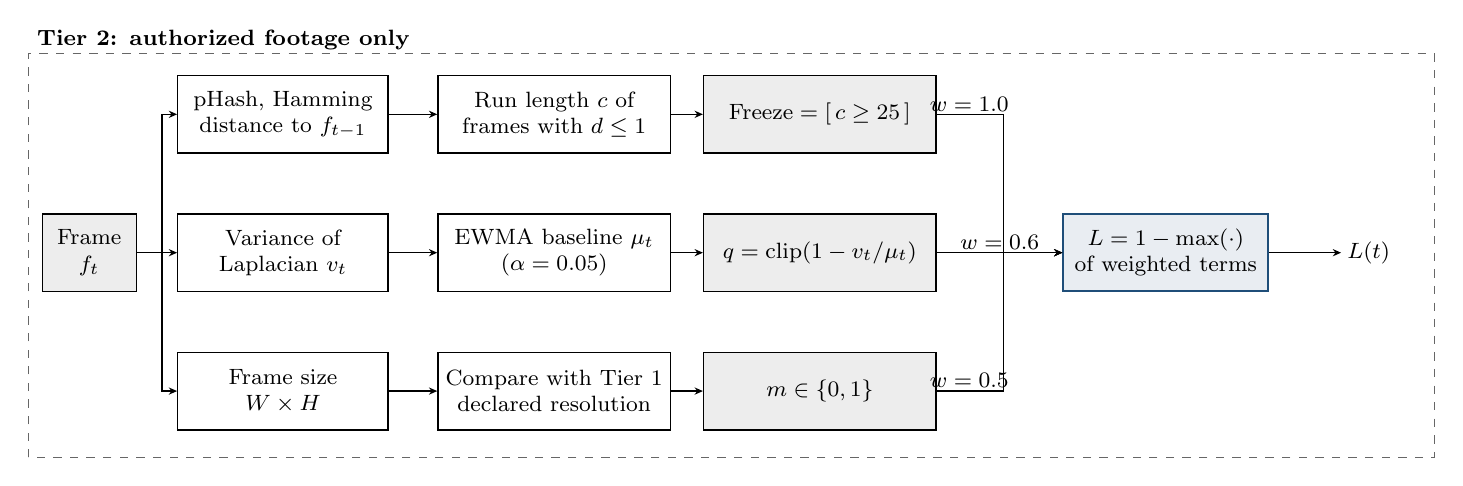
\begin{tikzpicture}[x=1pt,y=1pt]
  % boundary of the authorised-footage-only region
  \draw[dashed,line width=0.5pt,black!60] (2,-124) rectangle (510,22);
  \node[anchor=south west,inner sep=1pt,font=\footnotesize\bfseries] at (4,22) {Tier 2: authorized footage only};

  % input frame
  \node[frm] (F) at (24,-50) {Frame\\$f_t$};

  % branch 1: freeze
  \node[s1] (a1) at (94,0)    {pHash, Hamming\\distance to $f_{t-1}$};
  \node[s2] (a2) at (192,0)   {Run length $c$ of\\frames with $d\le 1$};
  \node[s3] (a3) at (288,0)   {$\mathrm{Freeze}=[\,c\ge 25\,]$};

  % branch 2: quality drift
  \node[s1] (b1) at (94,-50)  {Variance of\\Laplacian $v_t$};
  \node[s2] (b2) at (192,-50) {EWMA baseline $\mu_t$\\($\alpha=0.05$)};
  \node[s3] (b3) at (288,-50) {$q=\mathrm{clip}(1-v_t/\mu_t)$};

  % branch 3: spec mismatch
  \node[s1] (c1) at (94,-100)  {Frame size\\$W\times H$};
  \node[s2] (c2) at (192,-100) {Compare with Tier 1\\declared resolution};
  \node[s3] (c3) at (288,-100) {$m\in\{0,1\}$};

  % aggregation
  \node[agg] (mx) at (413,-50) {$L=1-\max(\cdot)$\\of weighted terms};

  % flows: frame to the three branches
  \draw[flow] (F.east) -- ++(9,0) |- (a1.west);
  \draw[flow] (F.east) -- (b1.west);
  \draw[flow] (F.east) -- ++(9,0) |- (c1.west);
  \foreach \r in {a,b,c}{
    \draw[flow] (\r1.east) -- (\r2.west);
    \draw[flow] (\r2.east) -- (\r3.west);
  }
  % flows: weighted bus into the aggregator
  \draw[flow] (a3.east) -- ++(24,0) |- (mx.west);
  \draw[flow] (b3.east) -- (mx.west);
  \draw[flow] (c3.east) -- ++(24,0) |- (mx.west);
  \node[wlab] at (342,0)   {$w=1.0$};
  \node[wlab] at (353,-50) {$w=0.6$};
  \node[wlab] at (342,-100) {$w=0.5$};

  % output
  \draw[flow] (mx.east) -- ++(26,0) node[right,inner sep=2pt] {$L(t)$};
\end{tikzpicture}
\end{document}
